\documentclass{article}
\usepackage[utf8]{inputenc}
\usepackage{graphicx}

\title{Assignment 3: Chess}
\author{Avery Frankenberg}
\date{January 21 2019}

\begin{document}

\maketitle

\section{Minimax and Cutoff Test}
The first step in this assignment was to implement a minimax algorithm. This algorithm is used often in 2 player games because we can easily represent one player trying to maximize their score to win and the other trying to minimize their score to win. This search relies on being able to search all the way until it reaches terminal states, otherwise known as leaf nodes. From searching until we get to these nodes, the algorithm then back propagates the values, alternating whether it prioritizes obtaining a maximum value or a minimum value. As the book describes, if the maximum depth of the tree is m and there are b different legal moves at each point then the time complexity of the algorithm is \(O(b^m)\). For a game like chess, this time complexity is far too large for the problem to be solved. Therefore, we must implement a cutoff test. For this first iteration of the algorithm, the cutoff test is whether a terminal state is reached (i.e. a win or a draw) or whether the maximum depth is reached (some arbitrary number assigned when the method is called). 

When I run this AI against the random AI it plays the same two moves over and over, g8h8 and then h8g8. This is because those are the first move that the algorithm checks and since all values except for the terminal states have a value of 0, there is no state that is better than these first vitied states and therefore the algorithm just moves back and forth between the two. However, once the evaluatin function is included in the minimax AI this should no longer occur. 

When testing the speed of this algorithm, it varies drastically based on the depth it is allowed to traverse to. When it runs with a maximum depth of 2, the call occurs almost instantaneously. It calls the minimax algorithm around 20 times and gets to a depth of 2 for each. When I called it on a maximum depth of 3, it takes at least double the time, but still is within the few seconds range which feels reasonable. It is still calling the minimax functionality around 20 times yet this time it goes down to a depth of 3. Increasing the maximum depth once again, the algorithm traversed down to a depth of 4 which increased the amount of time to around 60 seconds to make only one move. This demonstrates how expensive this algorithm can be, and how increasing the maximum depth by one can have a drastic affect on the amount of time each move takes. 

\section{Evaluation Function}
For the evaluation function I chose to create a material value heuristic. This type of heuristic values each of the different pieces and then sums up their value. I valued pawns as 1, knights and bishops as 3, rooks as 5, and queens as 9. In calculating the evaluation I then did the value of the white pieces minus the value of the black pieces and returned that value to the utility function which then returned to the minimax function.

\section{Iterative Deepening}
As discussed above, implementing a minimax algorithm for chess with no cutoff test is computationally unfeasible. However, in a chess game, each player has a time limit in which to move. If the time limit is reached before the minimax algorithm is complete, even using a cutoff test, there will be no next move to return. Therefore, the next step in this project was implementing iterative deepening. In this way, the AI will always have a next move ready. However, if given more time, it will continue to search further and further into the tree (deepening the search) generating more accurate and better next moves. For iterative deepening the same minimax algorithm is used; however, the method is called for a depth of 0, then 1, then 2, all the way to the overarching maximum depth value. In this way a move will always be ready, yet the minimax search can still run to the best of its ability. 

\section{Alpha-Beta Pruning}
Further improving our AI, I next implemented alpha-beta pruning. As the minimax algorithm has to search a number of nodes that is exponential to the depth of the tree, it is extremely time and space intensive. Although cutoff tests and iterative deepning help with this, they both limit the algorithm by restricting the depth to which it searches. Instead, alpha-beta pruning is a way to cut down the number of paths that are explored by a half. This means that alpha-beta pruning search algorithm can solve a tree to twice the depth that a minimax algorithm can.

After implementing alpha beta pruning, I tested it to see how deep it could search in a reasonable amount of time. I found that it could easily complete searches with a maximum depth of 4 in around the same amount of time that it took for minimax to complete a search with maximum depth of 3. With a maximum depth of 5, alpha beta still only took around 20-30 seconds to choose the next move, as compared to the minute that minimax took to search to a depth of 4. With these simple tests it is apparent how much deeper alpha beta can search as compared to minimax simply because of the ability to prune unhelpful branches. 

In addition, I tested alpha-beta against minimax to ensure that both algorithms were generating the same move with the same cost for the first move. I found that this was the case, as demonstrated below. You can see that both white (alpha-beta AI) and black (minimax AI) chose to move the knight on the right side of the board and that the score for this move is 0. This is one way to confirm that the algorithms are working correctly. 

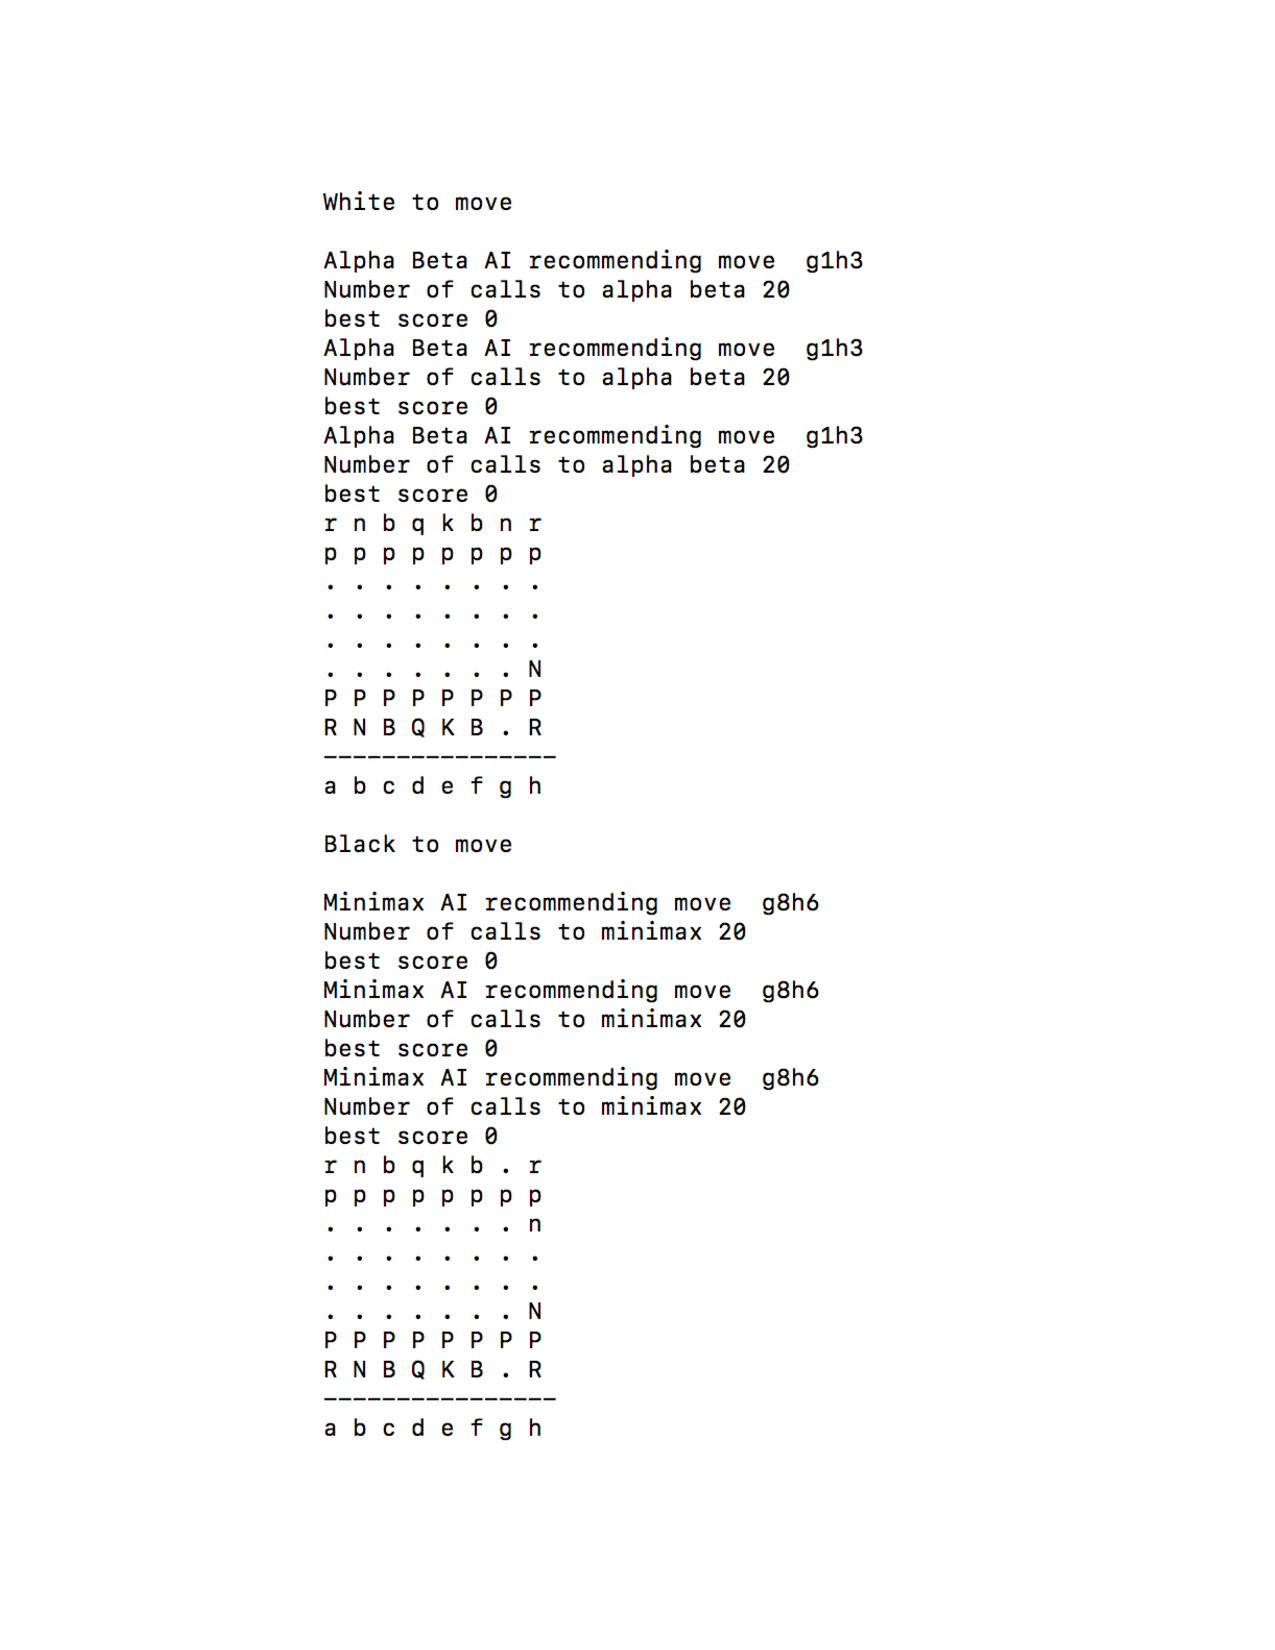
\includegraphics[width=\textwidth]{alpha-beta_vs_minimax.pdf}

After this set of tests, I included some move-reordering which improved the time it took to search by a bit. Instead of just searching all of the moves in the order that the legal moves method returns them, I checked for the moves that were captures first and checked their scores before moving on to the moves that didn't include captures. That is because often these moves are more beneficial for the player, so they are likely to generate a lower beta value and therefore allow for more pruning of the tree. More pruning means a smaller search tree to explore and therefore faster results. 

\section{Transposition Table}
For the transposition table, I created a dictionary which mapped strings of the board to their score. If the key was already explored, then the alpha beta algorithm wouldn't be called again and instead the score would be retrieved and output. This eliminates some searching because if a state is already evaluated it won't do it again. In addition, instead of just using the hash(str(game.board)) method to get the hash value, I created my own process board method. This method is explained further in the Bonus 6.1 section below.

This transposition table drastically affects the speed at which the algorithm runs. At the start when it is alternating between different states of cost 0 because no pieces have been captured yet it is much more efficient at returning a move because it doesn't have to calculate the score using alpha beta every time and instead can just return the score that was already obtained. Below is an example where the alpha beta AI had already explored the state where the subsequent move was h8g8. The first time it was explored, alpha beta was called twice, but after that it isn't called at all because the score is just obtained from the transposition table. This decreases the time the algorithm takes. 
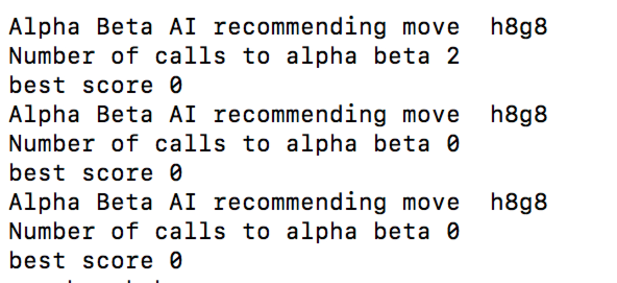
\includegraphics[width=\textwidth]{transposition_table.pdf}

\section{Bonus}

\subsection{Process board method}
This method takes only the locations of the pieces and who's turn it is and concatenates those values into a string which it then uses as the key for the dictionary. I decided to do this because I wanted board states to be considered the same despite the turn number. While the value of a transposition table explained in the book is to eliminate researching states reached via the same number of moves, but differently ordered moves. However, there are more states than this that are exactly the same as long as we disregard the number of moves. For this reason I chose to create my own process state method that reduces the string to only the pieces on the board and the player whose turn it is. 

\subsection{Literature Review}
After working on this chess AI I was interested in learning more about the other algorithms and improvements that have been generated and tested to date. I read one article in particular by David et.al. that discusses the creation of a deep chess algorithm that uses neural networks to train itself. I found this paper particularly interesting because they discussed how the most important part of the algorithm was the generation of a good evaluation function. In addition, they used an alpha-beta-esque algorithm; however, instead of using alpha beta values they used alpha position and beta position values. If a new position was better than the alpha or the beta then these position values would be updated, instead of the alpha beta scores we typically are updating. Similar to our algorithm, they hash states to ensure the same states aren't scored over and over again--thus saving time and memory. From their experiments David et.al. found that the deep neural network learned to favor moves that were considered dynamic attacking opportunities where pieces were sacrificed in the short term for long term gains. 

I found this article particularly interesting because it even though it is using a different technique than our AI algorithm (it is a form of genetic algorithm that incorporates learning into the intelligence), it emphasizes and tries to improve the same aspects. My algorithm focuses on creating an accurate evaluation function, alpha beta pruning, transposition tables, and move ordering--all aspects that this group of researchers hoped that their genetic algorithm would learn to optimize. 

Link to paper: https://www.cs.tau.ac.il/~wolf/papers/deepchess.pdf 

\subsection{Profiling}
For another extension I decided to profile my two algorithms, the AlphaBeta AI and the Minimax AI. I wrote the a file called bonus test profiling which does the profiling test for whichever algorithm you make player1. Pasted below are tables of some of the interesting results that I found. First, I thought it was extremely interesting how the AlphaBeta AI (including transposition tables and move reordering) was so much faster than Minimax and had substantially fewer total calls. This comparison is also clear when you compare individual method calls of the two algorithms. I didn't include min value, cutoff test, utility and evaluation from the AlphaBeta algorithm because those each had 1 call. However, Minimax had around 9,000 calls for each of these methods. The drastic difference between the two AI's is also mirrored in the general method calls such as piece at or append for lists. What these numbers of calls demonstrate is how many times the different algorithms are forced to check pieces or append lists, and therefore how many times the search algorithm was run. 

From the profiling that I did, I can clearly see why we chose to do move reordering and transposition tables in our AlphaBeta AI. However, I was unable to identify other areas from the AlphaBeta that specifically needed to be reduced. I list the calls that were called the most and the majority of these are general calls checking where pieces are or appending items to a list. Overall, this was an extremely interesting way to see at the ground level what is going on and how much we can improve an AI.



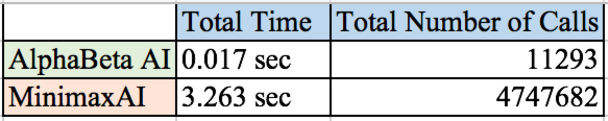
\includegraphics[width=\textwidth]{profiling_total.pdf}
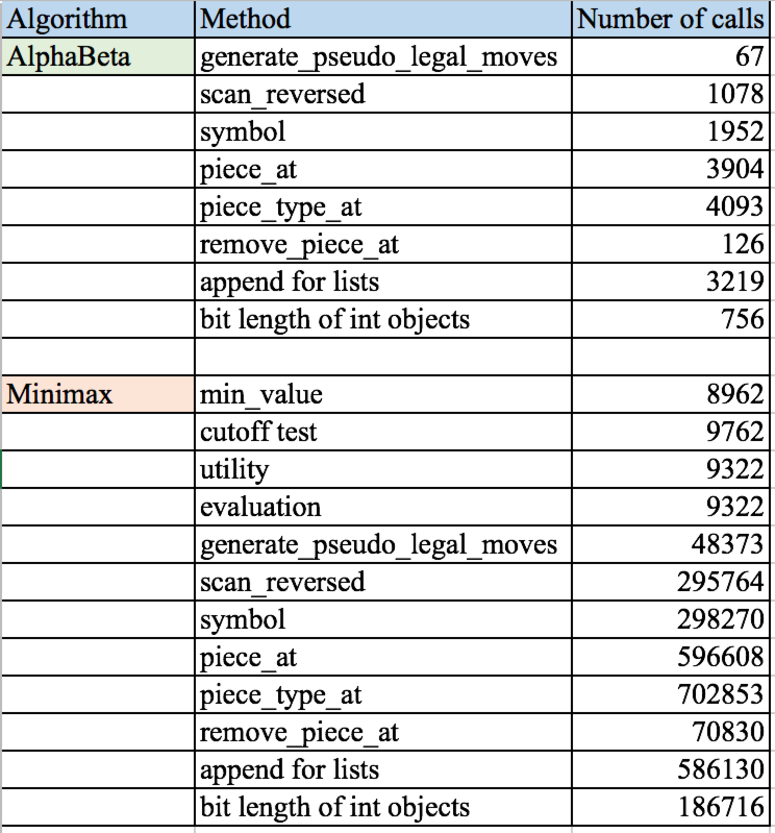
\includegraphics[width=\textwidth]{profiling_individualcalls.pdf}

\end{document}
